% Contained Is Not Closed -- main file.
% Build with `make` in paper/ (see paper/README.md). Do not edit venue.tex or
% macros-generated.tex by hand: both are written by the Makefile.
\documentclass[conference,10pt]{IEEEtran}

% ---- venue switch (generated: make agent | make icrito | make final) ----
\IfFileExists{venue.tex}{\input{venue.tex}}{%
  \newif\ifanon\anonfalse
  \newif\ificrito\icritofalse
  \newif\iffinal\finalfalse
  \newcommand{\PageLimit}{8}}

% ---- packages (IEEEtran-compatible only; nothing that changes margins, fonts or spacing) ----
\usepackage{cite}
\usepackage{amsmath,amssymb}
\usepackage{graphicx}
\usepackage{booktabs}
\usepackage{xcolor}
\usepackage{url}
\usepackage{siunitx}
\sisetup{group-separator={,},group-minimum-digits=4}
\usepackage{tikz}
\usetikzlibrary{positioning,arrows.meta}
\usepackage[hidelinks]{hyperref}   % load last

\graphicspath{{figs/}}

% ---- macros ----
% Hand-written paper macros. Keep this file tiny; numbers never go here.
% Draft mode: markers render in colour. Final mode (make final): every marker is a hard error.

\iffinal
  \newcommand{\MISSING}[1]{\errmessage{MISSING: #1}}
  \newcommand{\CONFIRM}[1]{\errmessage{CONFIRM: #1}}
  \newcommand{\CITEPENDING}[1]{\errmessage{CITEPENDING: #1}}
  \newcommand{\TODO}[1]{\errmessage{TODO: #1}}
\else
  \newcommand{\MISSING}[1]{\textcolor{red}{\textbf{[MISSING: #1]}}}
  \newcommand{\CONFIRM}[1]{\textcolor{orange}{[CONFIRM: #1]}}
  \newcommand{\CITEPENDING}[1]{\textcolor{red}{[CITE PENDING: #1]}}
  \newcommand{\TODO}[1]{\textcolor{blue}{[TODO: #1]}}
\fi

\newtheorem{proposition}{Proposition}

% \lit{...}: a literal that contains digits on purpose (e.g. scheduling notation).
% The number lint skips its argument; every use must be justifiable in review.
\newcommand{\lit}[1]{#1}
        % hand-written: \MISSING, \CONFIRM, \CITEPENDING, \TODO, \lit
\input{macros-generated.tex}    % generated: \input of every paper/generated/**/*.tex with macros
% Title, author and artifact macros. The ONLY place identifying information may appear.
% Section files must use \ArtifactURL etc., never literal names, handles or paths.

\newcommand{\PaperTitle}{Contained Is Not Closed: Evidence-Bounded Disposition and Safe Resumption of Remediation for Pre-Revocation Agent Payments}

\newcommand{\AuthorName}{Aditya Krishnan}
\newcommand{\AuthorAffil}{Independent Researcher}
\newcommand{\AuthorLocation}{Jersey City, NJ, USA}
\newcommand{\AuthorEmail}{aditya11997@gmail.com}
\newcommand{\RepoURL}{\url{https://github.com/aditya11997/contained-not-closed-artifact}}
\newcommand{\AnonArtifactURL}{\CONFIRM{anonymized artifact URL}}
% Zenodo record of the per-run holdout data (reserved DOI; resolves once the record is published).
\newcommand{\DataURL}{\url{https://doi.org/10.5281/zenodo.23650008}}
\newcommand{\AnonDataURL}{\CONFIRM{anonymized data URL}}

\ifanon
  \newcommand{\AuthorBlock}{\author{\IEEEauthorblockN{Anonymous Author(s)}}}
  \newcommand{\ArtifactURL}{\AnonArtifactURL}
  \newcommand{\DataLink}{\AnonDataURL}
  \hypersetup{pdfauthor={},pdftitle={\PaperTitle},pdfcreator={},pdfproducer={}}
\else
  \newcommand{\AuthorBlock}{\author{\IEEEauthorblockN{\AuthorName}
    \IEEEauthorblockA{\AuthorAffil\\ \AuthorLocation\\ \AuthorEmail}}}
  \newcommand{\ArtifactURL}{\RepoURL}
  \newcommand{\DataLink}{\DataURL}
  \hypersetup{pdftitle={\PaperTitle}}
\fi
                % title, author block, artifact link

\begin{document}

\title{\PaperTitle}
\AuthorBlock
\maketitle

% Written last. Rules (both venues): 150-250 words; objective -> method -> results -> conclusion;
% no citations; no abbreviations; numbers only via macros; says "single crash" and states the H3 null.
\begin{abstract}
When a software agent that makes payments is stopped, revocation prevents its next actions but not the payments it already created, which stay pending until the merchant captures them. An operator must cancel the suspect ones before capture, with limited capacity and an interface whose acknowledgments can be lost. We define a disposition contract that separates prevented, accounted-for and unresolved payments and lets a payment be reported as cancelled only on evidence from the payment processor. A pre-registered study of \NRunsPrimary{} primary simulator runs, each graded by an independent checker, then measures what that evidence costs. A runbook that trusts acknowledgments reports false closures in every configuration with transport faults, \FCShareAckHigh{} of its cancellation reports under high faults. Verifying each timeout before sending the next cancel costs loss when workers are scarce, whereas sending every cancel first and reconciling afterwards is never significantly worse than trusting acknowledgments and removes every false closure. Re-planning at every event adds nothing measurable. Restarted from a write-ahead journal behind idempotent cancels, evidence-bounded remediation survives a single crash per episode at every instrumented point, with no false closure or duplicate effect. The simulator's transitions match the Stripe test environment, and a case study with a revoked language-model agent shows that the agent's own summary cannot close an incident. Containment is not closure: closure needs evidence, and evidence is cheapest when the remediator does not wait for it.
\end{abstract}

\begin{IEEEkeywords}
reliability engineering, autonomous agents, revocation, incident remediation, runtime assurance
\end{IEEEkeywords}

% Budget: 0.90 pp (AGENT) / 0.70 pp (ICRITO), together with title and abstract.
% Outline source: docs/PAPER_OUTLINE.md section 1; REVAMP_PLAN section 1 (contribution 3 struck at G2).
\section{Introduction}\label{sec:intro}

Agents now place orders and initiate payments on behalf of people and firms, and agent payment protocols sign the mandates that authorize them~\cite{aviv2026ap2}. When such an agent misbehaves, the first response is to revoke it. Revocation stops what the agent does next. It does not stop what the agent already did: payments it created before the stop are held under manual capture~\cite{stripe2026hold} and become final when the merchant captures them, minutes or days later.

Someone has to dispose of those payments. In practice, a separate remediation authority cancels the suspect ones before capture, with a few operators, cancel calls that take time, and a processor interface whose replies are sometimes lost. Operations tooling then reports the incident closed. If it counts a cancel as done once it has been sent, it can report as prevented a payment that the merchant captured. Liu et al.\ showed that a transport acknowledgment does not establish that a revocation completed~\cite{liu2026revocation}. The same holds for the remediator's own calls, and it raises a question that their contract leaves open: once the agent is contained, what does it cost to close the incident only on evidence, under deadlines?

We answer with a contract, a pre-registered benchmark and a crash study:
\begin{itemize}
  \item A \emph{disposition contract} for pre-revocation effects with finality deadlines. It separates prevented, accounted-for and unresolved payments and admits a closure only on processor-side evidence; under a stated reply-integrity assumption, a report that obeys it contains no false closure (Section~\ref{sec:model}).
  \item A measured \emph{cost of assurance}. Across \NRunsPrimary{} primary runs graded by an independent checker, a runbook that trusts acknowledgments closes falsely in every faulty cell. Verifying each timeout before the next cancel costs loss when workers are scarce, while reconciling after all cancels are sent is never significantly worse and closes nothing falsely. Adaptive re-planning adds nothing measurable, a pre-registered null (Section~\ref{sec:results}).
  \item \emph{Safe resumption of remediation}: restarted from a write-ahead journal behind processor-side idempotency, evidence-bounded runbooks survive one crash per episode at every instrumented call point (Section~\ref{sec:results:h5}).
  \item A reproducible artifact: simulator, independent checker, Stripe test-mode conformance suite and a case study with a revoked language-model agent (Section~\ref{sec:casestudy}).
\end{itemize}

The closest work addresses neighbouring questions. Liu et al.\ decide when revocation is complete~\cite{liu2026revocation}; we start where their contract ends. Bhadane et al.\ re-check an approval before dispatch~\cite{bhadane2026runtime}; we handle what was dispatched before the stop. Wu et al.\ attack checkpoint and rollback of the agent itself~\cite{wu2026safe}; we resume the remediator. Section~\ref{sec:related} positions the rest. Scheduling is not a contribution: the Lawler--Moore algorithm~\cite{lawler1969functional} is our baseline.

% Budget: 1.20 pp (AGENT) / 0.90 pp (ICRITO).
% Sources: docs/REVAMP_PLAN.md section 2; p4/contract.py; p4/sim/protocol.py; p4/runbooks/base.py;
% p4/journal.py; checker/check.py (_check_report, _check_effect); docs/STRIPE_MAPPING.md.
% Fully symbolic: parameter VALUES (fault presets, slack, c, k, n) belong to Section IV.
\section{Problem Model and Disposition Contract}\label{sec:model}

An agent that is revoked mid-run stops creating effects, but the effects it created before the stop keep moving toward finality. We model that residue and state what a remediator must show before it may call an incident closed.

\subsection{Pending effects after revocation}\label{sec:model:effects}
Revocation happens at time \lit{$t_0 = 0$}. Before it, the agent created payments \lit{$i \in \{1,\dots,n\}$} under manual capture: each is authorized and held, and the merchant captures it later~\cite{stripe2026hold}. Payment $i$ has an amount $a_i$, a nominal capture time $d_i$ and a risk score $p_i$, all observed by the remediator, and a remediation permission $\pi_i$. Its actual capture time $D_i = d_i + \varepsilon_i$ and its label $y_i \in \{\text{suspect}, \text{legit}\}$ are hidden; the jitter $\varepsilon_i$ may be negative, so a capture can arrive early. Times are abstract simulation units, not card-network deadlines.

We take containment as given: after \lit{$t_0$}, every call by the revoked identity is denied, so it commits no new effect, which is condition C5 of Liu et al.~\cite{liu2026revocation} for this agent. Their contract decides when revocation is complete. Ours begins at that point and asks what is still open.

\subsection{Remediator, sink and transport faults}\label{sec:model:faults}
A separate remediation authority may cancel and read, but never create or capture. It runs $k$ parallel workers; a cancel occupies a worker for $s_i$ units (approval plus call) and a status read for $q$ units, and $k = \infty$ serves as a control.

The processor (the \emph{sink}) owns the clock and an append-only, hash-chained event log. A cancel applied before $D_i$ moves the payment from \textsc{pending} to \textsc{cancelled}; at $D_i$ a still-pending payment becomes \textsc{captured}. Both states are absorbing, since refunds and disputes lie outside the model. Idempotency keys are scoped to the calling actor and bound to the request: replaying a key returns the stored result without a second effect, and a key reused for a different request is an error, as in Stripe's API~\cite{stripe2026idempotency}. A replay is therefore also a status probe.

Between remediator and sink, a transport fault layer acts on each call. Under \texttt{drop\_req}, the request never arrives. Under \texttt{drop\_resp}, the sink commits but the reply is lost: a lost acknowledgment. During an outage window, calls time out, the sink commits a cancel with probability $r$, and status reads fail. One property holds throughout:

\smallskip
\noindent\textbf{Reply integrity.} \emph{Faults delete or delay replies; they never alter a reply that is delivered.}
\smallskip

\noindent The remediator itself may crash at any of four points of a call: before sending, after sending, after receiving the reply, or after journaling it. It keeps a write-ahead journal that records each intent before sending and each result after the reply. A restarted instance rebuilds its state from the journal, re-plans from the current time, and treats an intent without a recorded result as a timeout. Each payment has one fixed cancel key per incident, so a re-sent cancel cannot create a second effect.

\subsection{Loss and false closure}\label{sec:model:loss}
Let $\mathcal{C}$ and $\mathcal{X}$ be the payments whose log ends in \textsc{cancelled} and \textsc{captured}. The loss of an episode is
\begin{equation}\label{eq:loss}
  \textstyle L \;=\; \sum_{i \in \mathcal{X},\, y_i = \text{suspect}} a_i \;+\; c \sum_{i \in \mathcal{C},\, y_i = \text{legit}} a_i ,
\end{equation}
where $c$ weighs collateral cancellation of legitimate payments. Only the evaluator sees $y_i$ and computes $L$; runbooks never do. A \emph{false closure} is a report of \textsc{closed\_cancelled} for a payment whose log holds no \textsc{cancelled} effect before $D_i$. A \emph{false exposure} is a report of \textsc{closed\_exposure} for a payment that was never captured.

\subsection{Disposition contract}\label{sec:model:contract}
At a horizon after the last capture time, a runbook returns one disposition per payment (Table~\ref{tab:states}). Each closed entry carries two log sequence numbers: the line of the reply or read it relies on, and the \textsc{cancelled} or \textsc{captured} effect line that reply reports.

\begin{table}[t]
\centering
\scriptsize
\caption{Disposition states and the evidence an evidence-bounded runbook needs for each.}
\label{tab:states}
\begin{tabular}{@{}lll@{}}
\toprule
State & Meaning & Required evidence \\
\midrule
\textsc{closed\_cancelled} & prevented & reply, replay or read $=$ \textsc{cancelled} \\
\textsc{closed\_exposure} & accounted for & reply, replay or read $=$ \textsc{captured} \\
\textsc{unresolved\_pending} & open & last read $=$ \textsc{pending} \\
\textsc{unresolved\_unknown} & open & no definitive reply \\
\bottomrule
\end{tabular}
\end{table}

The \emph{evidence rule} binds the evidence-bounded runbooks (P4--P6): a payment may be closed only on a delivered sink reply, replay or status read that names the closing state. ACK-trust runbooks (P1--P3) may close without sink evidence: a timed-out cancel counts as success, and a payment they never attempted counts as captured at its nominal deadline. The first choice mirrors an operations dashboard that marks a job done once the cancel has been sent.

\begin{proposition}\label{prop:evidence}
Under reply integrity, a report whose closed entries all satisfy the evidence rule contains no false closure and no false exposure, including after a crash and restart from the journal.
\end{proposition}

\begin{IEEEproof}[Proof sketch]
The sink emits a \textsc{cancelled} reply or read only after it has written a \textsc{cancelled} effect, and it writes that effect only before $D_i$. Since the state is absorbing, it is still the final state at the horizon. By reply integrity, the delivered reply is the one the sink emitted, so a closure resting on it is true. The same argument covers \textsc{captured} and \textsc{closed\_exposure}. A restarted instance closes only on journaled results that pass the same rule, and it treats an intent without a result as a timeout, which closes nothing. The fixed cancel key makes any re-send a replay rather than a second effect.
\end{IEEEproof}

The proposition holds by construction, so zero false closures for P4--P6 verify the implementation; they are not an empirical discovery. The independent checker re-derives every disposition from the hash-chained log in a separate process (Section~\ref{sec:design}), and Section~\ref{sec:results:h5} tests the crash clause for one crash per episode. What the contract leaves open is the price: what evidence-bounded disposition costs in loss under deadlines, compared with trusting acknowledgments.

% Budget: 0.70 pp (AGENT) / 0.50 pp (ICRITO).
% Sources: docs/BASELINES.md; p4/sched/*.py; p4/runbooks/*.py; docs/PREREG.md section 3.
\section{Runbooks}\label{sec:runbooks}

Seven runbooks share one planning objective and differ in two independent choices: which cancels to attempt, and what they accept as proof (Table~\ref{tab:runbooks}). All of them receive the same observations, capacity, authority and fault realization for a given seed, and none can read $D_i$ or $y_i$; automated tests enforce both properties.

\subsection{Selection}
A planner targets permitted payments with positive expected gain \lit{$g_i = a_i\,(p_i - c\,(1-p_i))$}, and a cancel is feasible only if it completes before $d_i$. P1 accepts payments in earliest-deadline order while they remain feasible. P2 uses a weighted variant of Moore's algorithm~\cite{moore1968njob}: in deadline order, it drops the scheduled payment with the least gain per unit of work until the set is feasible, then refills. P3--P6 select with the Lawler--Moore dynamic program~\cite{lawler1969functional}, which is exact for the single-machine weighted tardy-jobs problem, that is, for $k = 1$. For \lit{$k > 1$} we keep the single-worker selection and list-schedule it across workers in deadline order with a fill pass, which is a heuristic. Since P3--P6 share this scheduler, every contrast among them holds scheduling fixed and isolates the evidence rule. Section~\ref{sec:results:sched} reports what a different heuristic does to absolute loss at $k = 4$.

\begin{table}[t]
\centering
\scriptsize
\setlength{\tabcolsep}{4pt}
\caption{Runbooks. All closures by P4--P6 rest on sink evidence (Section~\ref{sec:model:contract}).}
\label{tab:runbooks}
\begin{tabular}{@{}lll@{}}
\toprule
ID & Selection & Execution and closure rule \\
\midrule
P0 & none & no calls; reports exposure after $d_i$ \\
P1 & earliest deadline & ACK-trust: reply or timeout closes \\
P2 & weighted Moore & ACK-trust \\
P3 & Lawler--Moore & ACK-trust \\
P4 & Lawler--Moore & verify each timeout before the next cancel \\
P5 & Lawler--Moore & fire all, then replay timeouts (reconcile) \\
P6 & Lawler--Moore, re-planned & P5 with per-event re-planning \\
\bottomrule
\end{tabular}
\end{table}

\subsection{Execution and evidence}
The ACK-trust runbooks P1--P3 send their planned cancels in order and treat a \textsc{cancelled} reply or a timeout as success; a too-late reply or an unplanned payment counts as exposure. P4--P6 apply the evidence rule and differ only in when they seek proof.

\emph{Verify-each} (P4) resolves a timeout before its worker moves on: it reads the status until the answer is definitive or $d_i$ passes, and re-sends the same key if the payment is still pending and the cancel still fits. Its assurance is synchronous, so a timeout costs worker time.

\emph{Reconcile-after} (P5) fires every planned cancel first, then replays each timed-out cancel with its key until a definitive reply arrives or $d_i$ passes. This is the compensate-then-reconcile pattern of sagas~\cite{garciamolina1987sagas}, and the replay is safe because the processor returns the stored result for a known key~\cite{stripe2026idempotency}.

\emph{Adaptive} (P6) is P5 plus re-planning: at every free-worker event it re-solves Lawler--Moore over the payments not yet attempted, using the actual times at which workers become free. It has no free parameters, and its design was fixed on development seeds before the holdout runs.

After the last nominal capture time, P4--P6 run an accounting sweep, one status read per open payment, retried on timeout. With late cancellation, a sweep read that still finds a permitted, positive-gain payment pending triggers a cancel with the same key, because jitter can push a capture past $d_i$. P3 has neither the sweep nor late cancellation; we keep it that way because it is the frozen baseline, and the ablation in Section~\ref{sec:results:h1} bounds the effect.

After a crash, every runbook restarts from its journal. P1--P3 re-send an intent that has no recorded result once, with its key (outbox recovery); P4--P6 treat it as a timeout and resolve it with sink evidence.

% Budget: 0.80 pp (AGENT) / 0.55 pp (ICRITO).
% Sources: docs/PREREG.md sections 4-5 (frozen, tag prereg-v1); configs/*.toml (via design.tex);
% analysis/stats.py; checker/; tests/checker_mutation; scripts/verify_archive.py.
\section{Experimental Design}\label{sec:design}

\subsection{System under test}
Fig.~\ref{fig:arch} shows the harness. The sink owns the clock and writes every request, reply and effect to a hash-chained log; a capture emulator captures each pending payment at its hidden $D_i$. The fault layer draws its faults from a generator keyed by the seed and by each payment's call index, so every runbook meets the same fault realization. Runbooks see only observations and the processor protocol, and static tests forbid them from importing simulator internals or reading hidden labels. An independent checker runs as a separate process, imports only the shared log schema and none of the runbook code, and re-derives every disposition from the log and the hidden truth: it counts false closures, false exposures and duplicate effects and verifies the log's integrity. Mutation tests confirm that it flags each injected tampering of logs and reports. The same protocol is implemented by a Stripe test-mode adapter (Section~\ref{sec:casestudy}).

\begin{figure}[t]
  \centering
  % Fig. 2: system architecture. Hand-drawn TikZ (a diagram, not data); \input from 04-design.tex.
% Components and arrows follow p4/ (sim, runbooks, journal, adapters), checker/ and agent/.
\begin{tikzpicture}[
  font=\scriptsize,
  box/.style={draw, rounded corners=1.5pt, align=center, inner sep=2pt, text width=15mm, minimum height=7mm},
  arr/.style={-{Latex[length=1.5mm]}, semithick},
  lbl/.style={font=\tiny, inner sep=1pt}
]
% row 1
\node[box] (agent) at (2.15, 0) {agent or\\scenario};
\node[box] (cap) at (6.5, 0) {capture\\emulator};
% row 2
\node[box] (jr) at (0, -1.45) {write-ahead\\journal};
\node[box] (rb) at (2.15, -1.45) {runbook\\P0--P6, $k$};
\node[box] (fault) at (4.3, -1.45) {transport\\faults};
\node[box, minimum height=9mm] (sink) at (6.5, -1.45) {sink: sim or\\Stripe test\\mode; log};
% row 3
\node[box] (rep) at (2.15, -2.95) {disposition\\report};
\node[box] (chk) at (4.3, -2.95) {independent\\checker};
\node[box, dashed] (truth) at (6.5, -2.95) {hidden\\$D_i$, $y_i$};

\draw[arr] (agent) -- node[lbl, right] {observations} (rb);
\draw[arr, {Latex[length=1.5mm]}-{Latex[length=1.5mm]}] (jr) -- node[lbl, above] {} (rb);
\draw[arr] ([yshift=1mm]rb.east) -- ([yshift=1mm]fault.west);
\draw[arr] ([yshift=-1mm]fault.west) -- ([yshift=-1mm]rb.east);
\draw[arr] ([yshift=1mm]fault.east) -- ([yshift=1mm]sink.west);
\draw[arr] ([yshift=-1mm]sink.west) -- ([yshift=-1mm]fault.east);
\draw[arr] (cap) -- node[lbl, right] {at $D_i$} (sink);
\draw[arr] (rb) -- (rep);
\draw[arr] (rep) -- (chk);
\draw[arr] (sink.south west) ++(1mm,0) -- node[lbl, above, sloped] {log} (chk.north east);
\draw[arr, dashed] (truth) -- (chk);
\draw[arr, dashed] (truth.east) -- ++(1.5mm,0) |- (cap.east);
\node[lbl, below=0.6mm of chk, text width=30mm, align=center] {false closures, duplicate effects, invariants};
\node[lbl, below=0.3mm of jr, text width=17mm, align=center] {intent, result;\\restart};
\node[lbl, above=0.3mm of fault] {cancel, read, replies};
\end{tikzpicture}

  \caption{Harness. Runbooks reach the sink only through the fault layer; the checker grades every run from the log and the hidden truth.}
  \label{fig:arch}
\end{figure}

\subsection{Scenarios and grid}
Amounts lie between \DesignAmountMin{} and \DesignAmountMax{}, nominal capture times between \DesignDMin{} and \DesignDMax{} units scaled by a slack factor (\DesignSlackTight{} for tight, \DesignSlackNormal{} for normal), cancel costs between \DesignSMin{} and \DesignSMax{} units, and a status read costs \DesignQ{} unit. Risk scores between \DesignPMin{} and \DesignPMax{} are calibrated: payment $i$ is suspect with probability $p_i$. Remediation is permitted with probability \DesignPermitProb{}, capture jitter is uniform on $\{-j,\dots,j\}$ with $j = \DesignJitter$, and the collateral weight is $c = \DesignC$. The low fault preset sets $f_\mathrm{req} = \DesignFReqLow$, $f_\mathrm{resp} = \DesignFRespLow$ and outages at rate \DesignOutageRateLow{} of length \DesignOutageLengthLow; the high preset sets \DesignFReqHigh, \DesignFRespHigh, \DesignOutageRateHigh{} and \DesignOutageLengthHigh. Both commit a cancel during an outage with probability $r = \DesignOutageCommitHigh$. These values are sensitivity bands chosen on development seeds, not calibrated failure rates.

The primary grid crosses fault level (none, low, high), slack (tight, normal), $k$ (\lit{1, 4}) and $n$ (\lit{8, 32}): \DesignCells{} cells, \DesignPolicies{} runbooks and \NSeedsPrimary{} seeds per cell, \NRunsPrimary{} runs in total. Secondary blocks vary one factor at a time (score bias and noise, early-only jitter, $c$, $n = 128$, $k = \infty$ with faults, and late cancellation on or off at wider jitter; \NRunsSecondary{} runs). The negative control uses $k = \infty$ with no faults and no jitter (\NRunsNegativeControl{} runs). The crash matrix crashes the remediator at each of the four call points at the first pre-deadline cancel, at a call during an outage, at the first sweep read and at the first post-deadline cancel, then restarts it from its journal (\NRunsCrashMatrix{} runs).

\subsection{Pre-registration and statistics}
Every design choice was made on development seeds (\DesignDevFirst--\DesignDevLast). Hypotheses H1--H5 and C1, their decision rules and the analysis code were frozen under the git tag \texttt{prereg-v1} before any holdout seed ran, and the runner refuses holdout seeds without that tag. Holdout seeds come from the partition \DesignHoldoutFirst--\DesignHoldoutLast, and every cell and runbook receives the same \NSeedsPrimary{} seeds. The checker reported no integrity failure and no broken hash chain in any holdout run.

The primary outcome is per-seed loss (\ref{eq:loss}); contrasts are paired differences within a cell. We estimate means with a percentile bootstrap of \DesignBoot{} resamples and adjust the primary family, P4$-$P3 and P5$-$P3 in each of the \DesignCells{} cells, with the Holm--Bonferroni step-down procedure at $\alpha = \DesignAlpha$. H2 is decided by the Holm-level confidence bound; false-closure shares carry Wilson intervals. P6$-$P5 (H3) is a secondary analysis with unadjusted intervals. Analyses added after the holdout runs are labelled post hoc and decide nothing. Each was planned in writing before its code ran; PH8 was planned after its pattern had been noticed. PH2, PH3 and PH7 use development seeds, while PH5, PH6 and PH8 describe the holdout runs.

After a disk cleanup deleted holdout files, we regenerated them from the frozen commit. Today \ReproHoldoutFilesMatched{} of \ReproHoldoutFilesListed{} archived holdout files match their recorded \lit{SHA-256} hashes.

% Budget: 1.70 pp (AGENT) / 1.25 pp (ICRITO).
% Sources: paper/generated/verdicts.md; numbers.tex; posthoc.tex; contrasts_faulty_tex.tex (T4);
% crash_matrix.tex (T3); figs/f4_false_closure.pdf; docs/POSTHOC.md; docs/CHANGELOG_RESEARCH.md.
% Every number is a macro. Post-hoc results (PH2-PH8) are labelled in the text.
\section{Results}\label{sec:results}

All pre-registered verdicts follow from the frozen decision rules: H1, H2, H4, H5 and C1 are \VerdictHOne, and H3 is \VerdictHThree.

\subsection{Acknowledgment-trust closes falsely (H1)}\label{sec:results:h1}
P3 reports false closures in \NFaultyCellsAckFC{} of the \NFaultyCells{} faulty primary cells (Fig.~\ref{fig:falseclosure}). At low faults, \FCAckLow{} of its \FCClosedCancelledAckLow{} \textsc{closed\_cancelled} reports are false, a share of \FCShareAckLow{} (Wilson \lit{95\%} interval \FCShareLoAckLow--\FCShareHiAckLow); at high faults the share rises to \FCShareAckHigh{} (\FCShareLoAckHigh--\FCShareHiAckHigh). P1 and P2 also close falsely at both fault levels, and the pre-registered criterion for a negligible false-closure rate is \VerdictNegligibleFalseClosure. Each of these closures is a payment that a dashboard would show as stopped while the merchant captured it. P0 and P4--P6 report no false closure in any holdout run. That half of H1 holds by construction (Proposition~\ref{prop:evidence}); it verifies the implementation, and the checker's mutation tests show that a false closure would not go unseen.

P3 lacks the sweep and late cancellation that P4--P6 have (Section~\ref{sec:runbooks}). Switching late cancellation off for P4--P6 at jitter twice the primary value changes their mean loss by between $\AblLateCancelVerifyNoneTightJUniformSix$ and $\AblLateCancelVerifyHighNormalJUniformSix$ per run, small against the H2 effects below.

\begin{figure}[t]
  \centering
  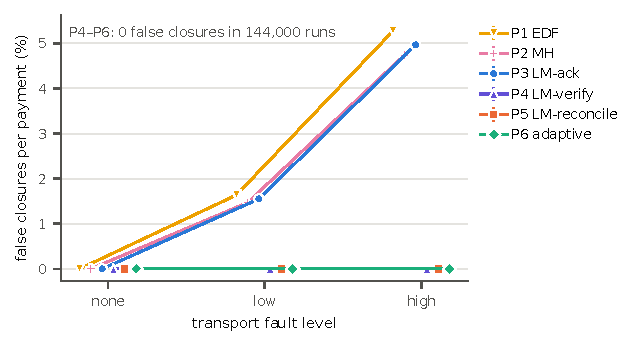
\includegraphics[width=0.92\columnwidth]{f4_false_closure}
  \caption{False closures per payment by fault level, primary grid. P0 and P4--P6 report none in any of their runs.}
  \label{fig:falseclosure}
\end{figure}

% Generated by analysis/report.py. Do not edit by hand.
% Holm family: every row of contrasts_primary.csv. The Holm CI is the percentile CI at level 1 - alpha/(m - rank + 1) (analysis/stats.py).
\begin{table}[t]
\centering
\scriptsize
\setlength{\tabcolsep}{4pt}
\caption{Paired loss differences in the 16 faulty primary cells (fault/slack/$k$/$n$): mean and CI at each contrast's Holm level. $^\dagger$\,Holm-adjusted $p \le 0.05$.}
\label{tab:contrasts-faulty}
\begin{tabular}{lrr}
\toprule
Cell & P4$-$P3 $\Delta$ [Holm CI] & P5$-$P3 $\Delta$ [Holm CI] \\
\midrule
low/tight/1/8 & 50.1 [22.0, 80.7]$^\dagger$ & $-$8.9 [$-$18.7, $-$1.0]$^\dagger$ \\
low/tight/1/32 & 158.7 [108.9, 211.3]$^\dagger$ & $-$6.5 [$-$15.8, 0.7] \\
low/tight/4/8 & $-$25.6 [$-$45.8, $-$7.0]$^\dagger$ & $-$35.9 [$-$57.6, $-$13.9]$^\dagger$ \\
low/tight/4/32 & 145.9 [84.9, 207.1]$^\dagger$ & $-$33.0 [$-$52.2, $-$15.3]$^\dagger$ \\
low/normal/1/8 & 48.5 [16.8, 85.0]$^\dagger$ & $-$8.6 [$-$19.6, 0.6] \\
low/normal/1/32 & 238.9 [175.0, 304.5]$^\dagger$ & $-$4.6 [$-$12.6, 1.8] \\
low/normal/4/8 & $-$43.2 [$-$67.9, $-$20.1]$^\dagger$ & $-$46.0 [$-$71.1, $-$22.1]$^\dagger$ \\
low/normal/4/32 & 113.3 [47.4, 180.1]$^\dagger$ & $-$39.9 [$-$61.0, $-$20.5]$^\dagger$ \\
high/tight/1/8 & 155.8 [107.7, 201.5]$^\dagger$ & $-$15.4 [$-$31.0, $-$1.8]$^\dagger$ \\
high/tight/1/32 & 427.9 [346.4, 515.1]$^\dagger$ & $-$13.2 [$-$25.3, $-$2.1]$^\dagger$ \\
high/tight/4/8 & $-$70.4 [$-$101.6, $-$38.6]$^\dagger$ & $-$117.0 [$-$154.8, $-$81.1]$^\dagger$ \\
high/tight/4/32 & 383.4 [302.3, 470.2]$^\dagger$ & $-$68.0 [$-$98.6, $-$39.0]$^\dagger$ \\
high/normal/1/8 & 165.9 [110.4, 218.9]$^\dagger$ & $-$24.5 [$-$43.4, $-$8.5]$^\dagger$ \\
high/normal/1/32 & 605.3 [515.7, 704.1]$^\dagger$ & $-$17.1 [$-$30.0, $-$5.8]$^\dagger$ \\
high/normal/4/8 & $-$143.7 [$-$185.2, $-$101.9]$^\dagger$ & $-$172.3 [$-$217.7, $-$129.8]$^\dagger$ \\
high/normal/4/32 & 428.5 [330.0, 522.0]$^\dagger$ & $-$86.4 [$-$116.9, $-$56.8]$^\dagger$ \\
\bottomrule
\end{tabular}
\end{table}


\subsection{The cost of assurance depends on when it is paid (H2)}\label{sec:results:h2}
Table~\ref{tab:contrasts-faulty} lists both pre-registered contrasts for the faulty cells. Verifying each timeout before the next cancel is expensive when workers are scarce. At tight slack, $k = 1$ and $n = 32$, P4 loses $\DiffVerifyAckLowTightKOneNThirtyTwo$ more than P3 at low faults and $\DiffVerifyAckHighTightKOneNThirtyTwo$ more at high faults, with Holm-level lower bounds of $\HTwoMinHolmLoLow$ and $\HTwoMinHolmLoHigh$; H2 is supported. Across the Holm family, P4 is significantly worse than P3 in \NHolmHigherVerifyAck{} cells and better in \NHolmLowerVerifyAck.

Reconcile-after behaves differently. P5 is never significantly worse than P3 (\NHolmHigherReconcileAck{} cells) and is significantly better in \NHolmLowerReconcileAck{} cells, all of them faulty, while reporting no false closure. Its timed-out cancels wait in a queue instead of blocking a worker, and a replay doubles as a status probe, so the evidence arrives late but costs little. In this model, then, assurance costs loss when it is synchronous and is close to free when it is deferred.

Four post-hoc analyses qualify this result.
\emph{Timeout cost (PH3, development seeds).} The simulator returns a timeout as fast as a reply. When timeouts take $m$ times as long, P4$-$P3 at H2's cells falls from $\PHThreeVerifyAckLowMOne$ to $\PHThreeVerifyAckLowMFour$ (low) and from $\PHThreeVerifyAckHighMOne$ to $\PHThreeVerifyAckHighMFour$ (high) as $m$ grows from one to four, because P3 also waits out its own timeouts. P5's advantage shrinks with it: at $k = 1$, $n = 32$, the interval of P5$-$P3 lies entirely below zero in \PHThreeReconcileAckKOneNThirtyTwoMOneCellsBelow{} of \PHThreeReconcileAckKOneNThirtyTwoMOneCells{} faulty cells at $m$ of one and in \PHThreeReconcileAckKOneNThirtyTwoMFourCellsBelow{} at $m$ of four.
\emph{Simultaneous intervals (PH6).} With Bonferroni-level intervals over the family of \PHSixFamilySize, the H2 lower bounds remain $\PHSixBonfLoVerifyAckLow$ and $\PHSixBonfLoVerifyAckHigh$.
\emph{Where P4 wins (PH5).} The \PHFiveCellsVerifyBetter{} cells where P4 beats P3 are the faulty cells at $k = 4$, $n = 8$. There, re-sending a timed-out cancel recovers between \PHFiveResendShareHighNormalKFourNEight{} and \PHFiveResendShareLowTightKFourNEight{} of the difference (above full when other effects push the other way): retrying is free when workers are idle.
\emph{Retrying without evidence (PH2, development seeds).} A variant of P3 that retries every timeout but still trusts acknowledgments (P3b) lowers the false-closure share to \PHTwoFCShareAckRetryLow{} (low) and \PHTwoFCShareAckRetryHigh{} (high) from P3's \PHTwoFCShareAckLow{} and \PHTwoFCShareAckHigh{} on the same seeds. P5 is below P3b in \PHTwoReconcileAckRetryCellsBelow{} of \PHTwoReconcileAckRetryCells{} faulty cells and above it in none. Retrying reduces false closures; only evidence removes them.

\subsection{The shared scheduler at \texorpdfstring{\lit{$k > 1$}}{multiple workers} (PH8, post hoc)}\label{sec:results:sched}
All contrasts above hold the scheduler fixed. Absolute loss does not: at $k = 4$, $n = 32$, the mean of P2$-$P3 ranges from $\PHEightMhAckMinAllKFourNThirtyTwo$ to $\PHEightMhAckMaxAllKFourNThirtyTwo$ per run across fault and slack levels, faultless cells included, and P2$-$P5 from $\PHEightMhReconcileMinAllKFourNThirtyTwo$ to $\PHEightMhReconcileMaxAllKFourNThirtyTwo$: P2's weighted Moore heuristic has the lower loss. At $k = 4$, $n = 8$ the difference to P3 lies between $\PHEightMhAckMinAllKFourNEight$ and $\PHEightMhAckMaxAllKFourNEight$. The lowest-loss runbook in those larger cells is therefore an ACK-trust one, and it still closes falsely (\FCMhHigh{} false closures over the high-fault cells). Lawler--Moore is exact only at $k = 1$, and an evidence-bounded runbook on a stronger multi-worker scheduler was not part of the study.

\subsection{Adaptive re-planning and the control (H3, H4)}\label{sec:results:h3h4}
Re-planning at every free-worker event adds nothing measurable to reconcile-after. At $k = 1$, P6 and P5 differ in loss on \HThreeNonzeroSeedsKOne{} of \HThreeSeedsKOne{} seeds. At $k = 4$ they differ on \HThreeNonzeroSeedsKFour{} of \HThreeSeedsKFour{} seeds, yet none of the \HThreeCellsKFour{} intervals excludes zero, so H3 is not supported, as development data had predicted. The negative control behaves as a sanity check should: with unlimited workers, no faults and no jitter, P3--P6 incur equal loss on \NegCtrlSeedsEqual{} of \NegCtrlSeeds{} seeds, since every runbook sends every planned cancel at once and every call succeeds.

% Generated by analysis/report.py. Do not edit by hand.
% Rows sum each policy's crash-matrix cells over all their runs, crashed or not.
% Crashed (min): crashed runs, and in parentheses the fewest crashed runs in one cell.
% FC/FE/Dup: false closures, false exposures, duplicate effects; Inv: runs with a failed invariant.
% A cell holds with FC = FE = Dup = Inv = 0 and at least 100 crashed runs (H5).
\begin{table}[t]
\centering
\scriptsize
\setlength{\tabcolsep}{4pt}
\caption{Crash matrix (H5), summed over each policy's cells. P3's false closures are measurements; P3 is not part of H5.}
\label{tab:crash-matrix}
\begin{tabular}{lrrrr}
\toprule
Policy & Cells held & Crashed (min) & FC & FE/Dup/Inv \\
\midrule
P3 & -- & 50{,}808 (2{,}808) & 21{,}644 & 0/0/0 \\
P4 & 13/13 & 114{,}500 (3{,}803) & 0 & 0/0/0 \\
P5 & 13/13 & 111{,}977 (3{,}170) & 0 & 0/0/0 \\
P6 & 13/13 & 111{,}769 (3{,}126) & 0 & 0/0/0 \\
\bottomrule
\end{tabular}
\end{table}


\subsection{Safe resumption of remediation (H5)}\label{sec:results:h5}
Table~\ref{tab:crash-matrix} summarizes the crash matrix. For P4--P6, all \HfiveCellsHold{} (cell, runbook) pairs hold: across \num{\HfiveCrashedRuns} crashed runs, with at least \num{\HfiveMinCrashed} per pair, the checker finds \HfiveFalseClosures{} false closures, \HfiveFalseExposures{} false exposures and \HfiveDuplicateEffects{} duplicate effects, and no failed invariant. The combination of a fixed cancel key, processor-side idempotency and the write-ahead journal therefore survives one crash per episode at every call point we instrumented. P3, which re-sends orphaned intents and trusts the reply, keeps closing falsely after a restart.

The claim covers one crash per episode. In a post-hoc run on development seeds with two crashes per episode (PH7), \PHSevenPairsHold{} of \PHSevenPairs{} pairs hold over \PHSevenCrashedTwice{} doubly crashed runs. The same exercise exposed a defect in the frozen P3: two crashes before one cancel's result is journaled leave two orphaned intents, and its outbox recovery fails. The holdout matrix crashes at most once per run, so no frozen result is affected; we leave P3 unchanged because it is the frozen baseline.

% Budget: 0.50 pp (AGENT) / 0.30 pp (ICRITO).
% Sources: paper/generated/stripe.tex; docs/STRIPE_MAPPING.md; paper/generated/case_study.tex;
% docs/CASE_STUDY.md (generated tables; outside the pre-registered contrasts; dev seeds).
\section{Processor Conformance and an Agent Case Study}\label{sec:casestudy}

\subsection{Stripe test-mode conformance (C1)}\label{sec:casestudy:c1}
A test-mode adapter implements the sink's protocol on Stripe PaymentIntents with manual capture: create, cancel with an idempotency key, status read, and merchant capture at $D_i$. For each mapped transition, the conformance suite drives the simulator and Stripe with identical payments on a shared logical clock and requires the two event logs to agree line by line, which makes their hash chains equal. All \StripeMappingRowsMatched{} of \StripeMappingRows{} mapped transitions matched, and \StripeTestsPassed{} of \StripeTestsRun{} conformance tests passed: \StripeTransitionScripts{} transition scripts and \StripeEpisodes{} whole episodes of P3, P5 and P6 with and without faults. Two documented behaviors carry the model. A cancel after capture fails, and the stored error is returned again for the same key; after a lost acknowledgment, a replay with the same key returns the stored cancellation without a second effect, as documented~\cite{stripe2026idempotency} and observed live. C1 is \VerdictCOne. Its scope is narrow: live fault injection covered lost acknowledgments only, and test mode is not live mode.

\subsection{A revoked LLM agent}\label{sec:casestudy:agent}
\begin{figure*}[t]
  \centering
  \includegraphics[width=0.82\textwidth]{fig1_timeline}
  \caption{One case-study run on Stripe test mode. Before the stop (left, in call order) the agent creates four payments; the mandate wrapper rejects an over-limit purchase. At the stop the revoked agent's remaining calls are denied. P6 cancels one flagged payment before capture and closes the captured ones on status reads, each on processor evidence.}
  \label{fig:timeline}
\end{figure*}
To show the chain end to end (Fig.~\ref{fig:timeline}), a local \texttt{\CaseStudyModel} model drives a procurement agent through a minimal tool-calling loop. A brief asks it to buy a list of items; budget, vendor allowlist and per-purchase maximum are enforced in deterministic code, not by the model. After a fixed number of successful purchases, the harness revokes the agent while its loop is still running. Its remaining calls are denied and logged, and the checker finds \CaseStudyRevokedActorEffects{} revoked-actor effects. P6 then disposes of the pending payments on Stripe test mode or on the simulator, and in each of the \CaseStudyRuns{} runs its live dispositions equal those of a simulator replay. In \CaseStudySummariesOmitStop{} of \CaseStudyRuns{} runs, the agent's closing summary never mentions the revocation or a denied call, and some summaries list as placed purchases that the log shows were denied. The agent's account of its own work cannot close an incident; the processor's log can. With few payments, $k = 1$ and low faults, P3, P5 and P6 reach the same dispositions here, which says nothing about their differences.

% Budget: 0.60 pp (AGENT) / 0.45 pp (ICRITO).
% Placed after the evidence (decision 2026-10-24); the introduction carries a closest-work paragraph.
% Every \cite key is logged in docs/REFERENCES_VERIFIED.md (make check enforces it).
\section{Related Work}\label{sec:related}

\emph{Revocation and authority.} Liu et al.\ separate issuer commit, transport acknowledgment, receiver persistence, gateway enforcement and effect prevention, and certify revocation only at the last stage~\cite{liu2026revocation}; that acknowledgment is not completion is their observation, which we carry over to the remediator's own calls. VERA computes which agents lose authority when one delegation edge is revoked~\cite{liu2026vera}. Both decide who may still act. We begin once that question is settled and ask what the agent's earlier actions left open.

\emph{Control before the effect.} Bhadane et al.\ bind an execution allowance to the basis of an approval and re-check it at dispatch~\cite{bhadane2026runtime}. They note that a lost acknowledgment can let a valid retry commit twice and leave compensation and reconciliation outside their guarantee, which is the space this paper measures. Peng and Wu identify stale authorization as the core failure when agents execute refunds and transfers, and coordinate policy state with effects~\cite{peng2026stateful}. These mechanisms govern effects before dispatch; ours governs those already dispatched when the stop arrives.

\emph{Recovery and rollback.} Wu et al.\ show that restoring an agent checkpoint can resume an execution whose external effects were never recorded, and demonstrate a double payment~\cite{wu2026safe}. Zhang and Liu treat recovery as an explicit decision, since retrying a tool call may duplicate its effect~\cite{zhang2026recoverability}. Our resumption concerns a different component: the remediator, restarted from a write-ahead journal behind processor-side idempotency, and graded by an independent checker.

\emph{Agent payments.} An analysis of the Agent Payments Protocol finds that a validly signed mandate can still encode an unintended payment when the context before signing is manipulated~\cite{aviv2026ap2}. Cryptographic authorization therefore does not remove the need to remediate after the fact.

\emph{Compensation and scheduling.} Sagas pair each step with a compensating transaction~\cite{garciamolina1987sagas}; P5 applies that pattern with reconciliation by replay. Choosing which cancels to attempt is weighted tardy-job scheduling, solved exactly on one machine by Lawler and Moore~\cite{lawler1969functional}, while Moore's algorithm solves the unweighted case and underlies P2's weighted heuristic~\cite{moore1968njob}. We use both as baselines and claim nothing new about them.

% Budget: 0.45 pp (AGENT) / 0.30 pp (ICRITO). Covers every item in docs/CHANGELOG_RESEARCH.md
% ("Threats to validity: not tested live" and "model and design") and the skill's list.
\section{Threats to Validity}\label{sec:threats}

\emph{Construct.} The zero false closures of P4--P6 hold by construction under reply integrity (Proposition~\ref{prop:evidence}); they verify the implementation. Stale or reordered status reads are not modelled, and a processor with eventually consistent reads could make an evidence-bounded runbook close falsely. Timeouts arrive as fast as replies, which favours runbooks that retry or verify; PH3 shows the direction and size of this effect on development seeds. The negative control (H4) checks plumbing, not the cost of assurance under failure.

\emph{Internal.} P3 has no accounting sweep and no late cancellation; the ablation bounds what late cancellation is worth. The frozen P3 fails after two crashes on one in-flight cancel; the holdout matrix never crashes twice. A static test against reading simulator clock internals was added after the freeze; it passes on the frozen runbooks. The experiment configurations share seed ranges, so their results are correlated. H5 covers one crash per episode; two crashes were tested only post hoc.

\emph{External.} Parameters are synthetic and fault presets are sensitivity bands. All results concern one payment processor's semantics. At \lit{$k > 1$} the shared scheduler is a heuristic that a different heuristic beats (Section~\ref{sec:results:sched}); an evidence-bounded runbook on the stronger heuristic was not pre-registered. Conformance holds for Stripe test mode, not live mode. Live fault injection covered lost acknowledgments only: dropped requests and outages, which cause every P3 false closure, were tested against the simulator, and rate-limit and server-error handling only against a mock. Capture timing used a logical clock except in the case study, and authorization expiry was never reached. The agent case study uses one local model and few runs, and a denied agent call during an episode was tested offline only.

% Budget: 0.20 pp (AGENT) / 0.15 pp (ICRITO).
% Future work: at most two sentences (Kill-and-Close framework is paper 2).
\section{Conclusion}\label{sec:conclusion}
Containing an agent ends its future actions; closing the incident requires accounting for its past ones. A runbook that equates a sent cancel with a stopped payment reports closures the processor contradicts. Requiring processor-side evidence removes those false closures, and in this model the price of that evidence depends on when it is sought: waiting for it before each next cancel costs loss under scarce capacity, collecting it after all cancels are sent costs little. Remediation that closes only on evidence also resumes safely after a crash, given a journal and idempotent cancels. Code and trial data are available at \ArtifactURL, and the per-run data behind every verdict at \DataLink. Joining revocation and disposition into one verified incident procedure is the next step.

% Budget: 0.15 pp (AGENT) / 0.10 pp (ICRITO). IEEE AI-generated content policy: identify the AI
% system, the sections that use AI-generated content, and the level of use, in the Acknowledgment
% (open.ieee.org/author-guidelines-for-artificial-intelligence-ai-generated-text, read 2026-10-25).
% Every statement about the author's role must be true; the author confirms before submission.
% Names no person or employer, so it stays unchanged under double-blind review.
\section*{Acknowledgment}
The author conceived the problem and the disposition contract, designed and pre-registered the study, specified and reviewed its implementation, and made the methodological and interpretive decisions reported here. In line with IEEE policy, the author notes that Anthropic's Claude was used as an assistant for parts of the code and for drafting and editing text across the sections; all such content was directed, reviewed, revised and verified by the author, who takes full responsibility for this paper.


\bibliographystyle{IEEEtran}
\bibliography{refs}

\end{document}
